\begin{frame}
    \frametitle{Skewness Analysis}
    \begin{itemize}
        \item \textbf{Formulas:}
        \[
        \begin{aligned}
        \text{Moments Skewness} &= \frac{\mu_3}{\sigma^3} \\
        \text{Pearson Skewness} &= \frac{3(\bar{x} - \tilde{x})}{\sigma} \\
        \text{Bowley Skewness} &= \frac{Q_1 + Q_3 - 2\tilde{x}}{Q_3 - Q_1}
        \end{aligned}
        \]
        
        \item \textbf{Results:}
        \begin{itemize}
            \item Moment Coefficient: 0.649
            \item Pearson's Skewness: 0.250
            \item Bowley's Skewness: 0.052
        \end{itemize}
    \end{itemize}
\end{frame}

\begin{frame}
    \begin{itemize}
        \item \textbf{What the Data Shows:}
        \begin{itemize}
            \item More countries with higher-than-average rates
            \item 15 countries have very high rates (over 80 cases)
            \item Example: Belgium (105 cases) vs average (48 cases)
        \end{itemize}
        
        \item \textbf{Why This Matters:}
        \begin{itemize}
            \item High-rate countries may need more healthcare resources
            \item Low-rate areas might have underreported cases
            \item Natural variation between countries is significant
        \end{itemize}
    \end{itemize}
\end{frame}

\begin{frame}
    \frametitle{Kurtosis Analysis}
    \begin{itemize}
        \item \textbf{Formula:}
        \[
        \text{Excess Kurtosis} = \frac{\mu_4}{\sigma^4} - 3
        \]
        
        \item \textbf{Result:}
        \begin{itemize}
            \item Excess Kurtosis: 0.241
        \end{itemize}
        
        \item \textbf{Interpretation:} Positive value indicates leptokurtic distribution (sharper peak than normal), suggesting clustering around mean with heavy tails of extreme values.
    \end{itemize}
\end{frame}

\begin{frame}
    \frametitle{Kurtosis Insights}
    \begin{itemize}
        \item \textbf{What the Data Shows:}
        \begin{itemize}
            \item More countries cluster around average rates (48 cases) 
            \item But also more extreme values than expected
            \item Examples from dataset:
                \begin{itemize}
                    \item High: Belgium (105 cases)
                    \item Low: Afghanistan (0 cases)
                \end{itemize}
        \end{itemize}
        
        \item \textbf{Why This Matters:}
        \begin{itemize}
            \item Most countries have moderate rates
            \item A few countries need special attention
            \item Data has "heavy tails" - unexpected extremes
        \end{itemize}
    \end{itemize}
\end{frame}

\begin{frame}
    \frametitle{Skewness Measures Comparison}
    \centering
    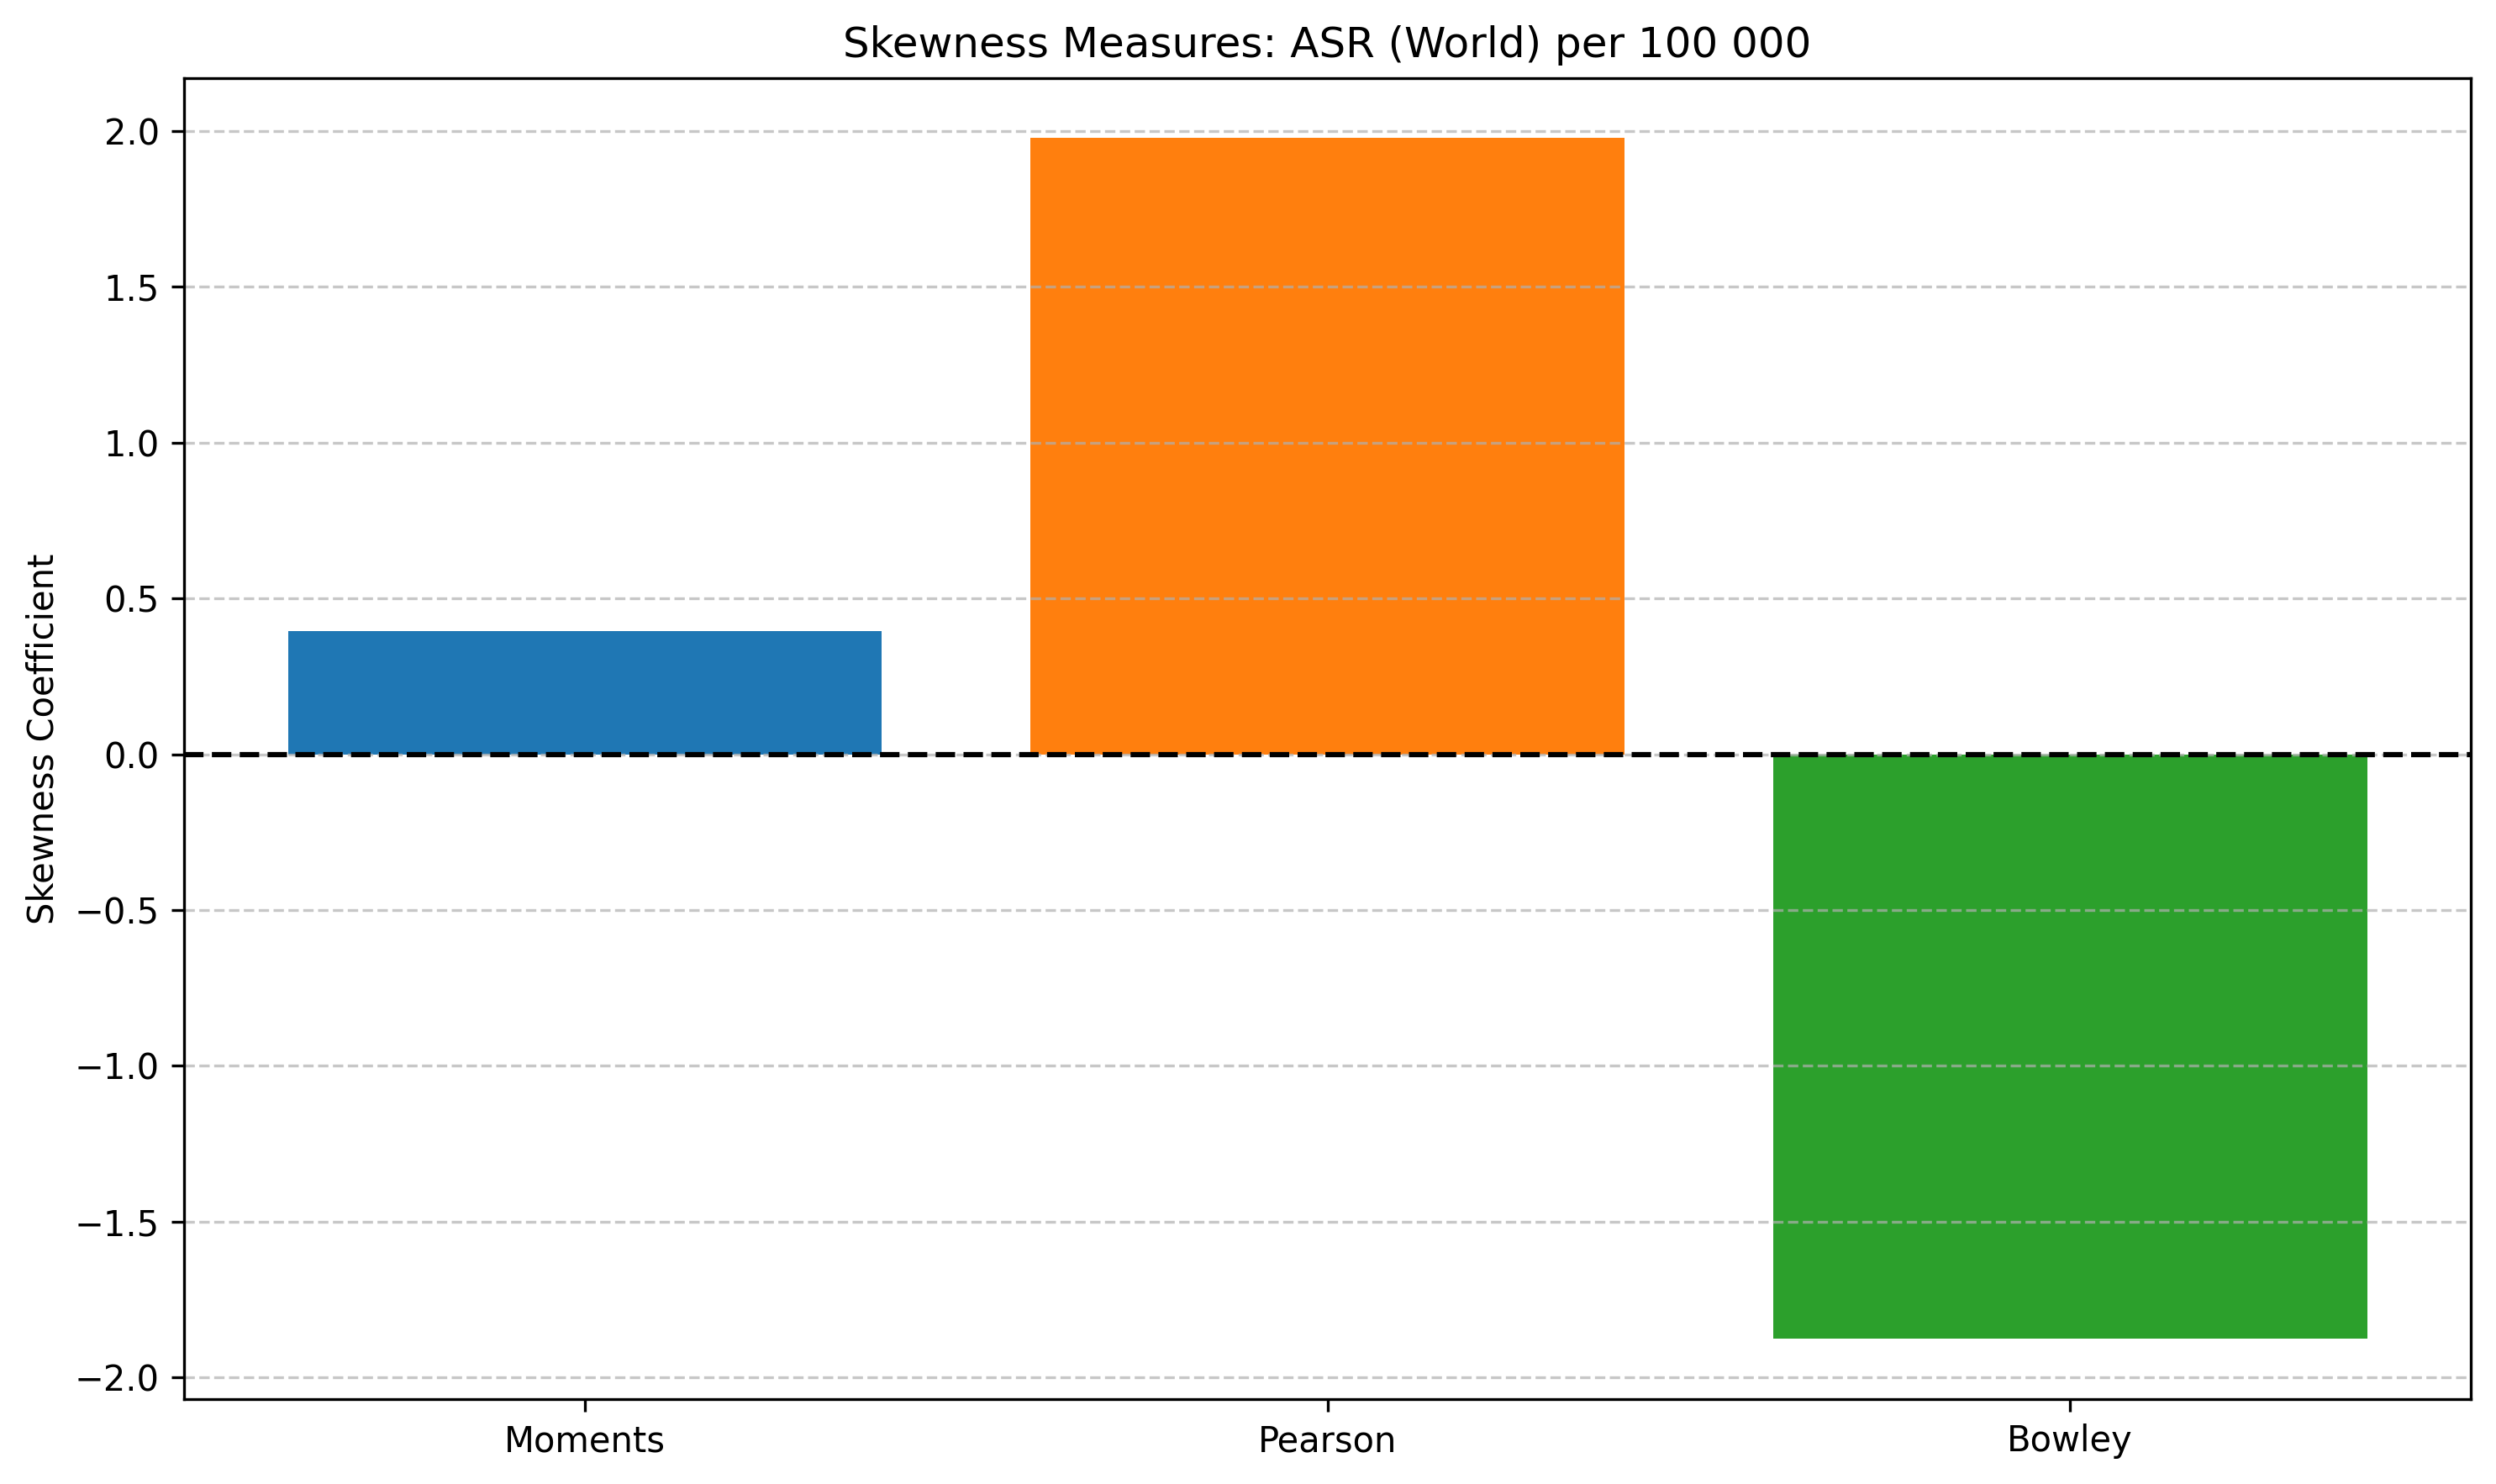
\includegraphics[width=0.75\textwidth,height=0.6\textheight,keepaspectratio]{images/graph/skewness_comparison.png}
    \vspace{-0.5em}
    \begin{itemize}
        \item \textbf{Key Observation:}
        \begin{itemize}
            \item Moment measure most sensitive to outliers
            \item Bowley's measure shows mild asymmetry in middle 50\% data
            \item All measures agree on positive direction of skew
        \end{itemize}
    \end{itemize}
\end{frame}

\begin{frame}
    \frametitle{Skewness Comparison Insights}
    \begin{itemize}
        \item \textbf{Key Findings:}
        \begin{itemize}
            \item All methods agree: More high-rate countries
            \item Outliers strongly affect some measures
            \item Middle-range countries show mild imbalance
        \end{itemize}
        
        \item \textbf{What This Means:}
        \begin{itemize}
            \item High-rate countries are true extremes
            \item Most countries cluster in lower half
            \item Data patterns are consistent across methods
        \end{itemize}
    \end{itemize}
\end{frame}